\chapter{Introduction}
\label{chap:intro}
\resetallacronyms

\begin{shaded}
  This chapter demonstrates why more efficient domestic heating systems
  are necessary and identifies why heat pumps are one of the best
  candidates for this improvement.
\end{shaded}

\section{The world energy consumption needs to be slowed down}
\label{sec:intro-slow-energy}


\paragraph{The world energy consumption increases dramatically.}In
slightly more than 40 years, the global energy consumption has almost
doubled. Indeed, from 1973 to 2012, the global final energy
consumption increased from 4672 Mtoe\footnotep{\label{Mtoe}Mtoe:
  Megatons petroleum equivalent.} to 8979 Mtoe\cref{Mtoe}
\citep[p.\,28]{iea-2014a}\index{energy consumption}. In order to
illustrate the growth at a more local scale,
\cref{fig:energy-consumption-ch-2012} presents the evolution of the
use of each energy source during the 20$^{\text{th}}$ century in
Switzerland. Since the end of the World War II, the energy consumption
follows a worrying trend. In a context where humanity starts to feel
the limits of the Earth resources, changing this trend is a necessity
everywhere on the planet.

\begin{figure}[htbp]
  \centering
  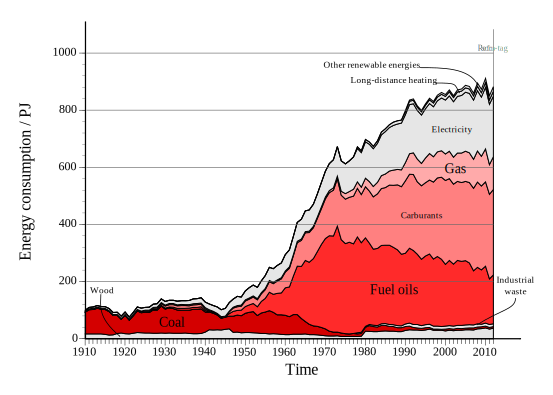
\includegraphics[height=10cm]{energy-consumption-switzerland-1910-2012-ofen-2012a-fig1p4}
  \caption[Final energy consumption in Switzerland]
  {Final energy consumption in Switzerland, based on the work of the
    \citet[Fig.\,1, p.\,4]{ofen-2012a}.}
  \label{fig:energy-consumption-ch-2012}
\end{figure}

\paragraph{The domestic sector represents about 30\% of the world
  final energy consumption} Investigating further this energy
consumption highlights that the worldwide domestic energy uses are
almost as high as the industry uses; they almost reach a third of the
global consumption and are mostly provided by fossil
fuels\index{energy consumption!fossil fuel consumption}. Indeed, the 3
big shares representing most of the global energy consumption are the
industry, with 33\% of the consumption, the domestic uses, with 29\%
(which are responsible of 21\% - 4.5 Gto of CO$_{2}$\index{carbon
  dioxide emissions} - of the carbon dioxide emissions), and the
transportation sector, with 26\%
\citep[p.\,17]{iea-2008a}\index{energy consumption}. Moreover, from
1973 to 2010, the ratio between the different fuels kept approximately
the same. The only significant exception concerns the transition from
coal to electricity \citep[p.\,28]{iea-2008a}, particularly motivated
by the development of the nuclear energy. During the period, natural
gas and oil consumption ratios also kept approximately
constant\index{energy consumption!fossil fuel consumption}. Global
energy use in the domestic sector increased between 1990 and 2005 by
19\%. Moreover, the domestic sector is the only major end-use sector
where the increase in energy consumption since 1990 has been greater
in OECD countries (+22\%) than in non-OECD countries (+18\%)
\citep[p.\,44]{iea-2008a}.


\paragraph{Space \& water heating represent about 70\% of the IEA19
  domestic sector energy consumption} In the IEA19
countries\footnotep{IEA19 is a set of 19 countries where extended
  energy data is available. Notably those 19 countries have domestic
  sector final energy consumption statistics available. The 19
  countries are Australia, Austria, Canada, Denmark, Finland, France,
  Germany, Ireland, Italy, Japan, Korea, Netherlands, New Zealand,
  Norway, Spain, Sweden, Switzerland, United Kingdom, United States of
  America.}, space heating remains the most important energy use,
responsible for 53\% of household final energy consumption, as
illustrated in \cref{fig:household-energy-consumption-2005}. This
share has decreased a bit (5\%) since 1990, but the energy saved has
been transferred to the appliance consumption. Space and water
heating, as illustrated in
\cref{fig:household-energy-consumption-2005}, make together an almost
stable consumption of about 70\% of the energy used in the domestic
sector over the last 25 years. Moreover, the share of the domestic
heating is considerably larger for the colder climates where space
heating demands higher temperature lifts, which are even higher for
the houses heated with conventional hydronic
systems\footnotep{Conventional hydronic systems may usually need
  water temperatures higher than 60\si{\degreeCelsius} while hydronic
  heating floor systems only need temperature up to
  35\si{\degreeCelsius}.}\index{energy consumption}.

\begin{figure}[htbp]
  \centering
  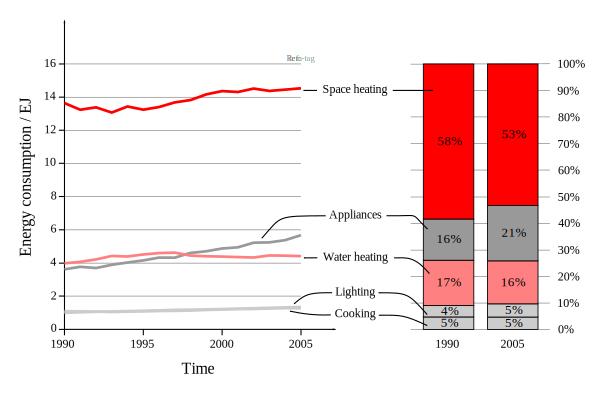
\includegraphics[height=10cm]{iea19-domestic-heating-iea-2008a-fig43p46}
  \caption[Final household energy consumption for the IEA19]
  {Final domestic sector energy consumption for the IEA19, based on
    the work of the \citet[Fig.\,4.3, p.\,46]{iea-2008a}.}
  \label{fig:household-energy-consumption-2005}
\end{figure}

\paragraph{Space \& water heating technologies for domestic uses}
Space and water heating is mostly performed around the world with fuel
consumption. The technologies involved are thermally-driven heat
pumps\index{heat pump!thermally-driven heat pump}, cogeneration,
fuel-cells, and of course, boilers. Direct electric heating is also
used, as is the use of electrically-driven heat pumps\index{heat
  pump!electrically-driven heat pump} (the latter still representing a
small share)\index{space \& water heating technologies}.

\paragraph{Heat pumps have a great potential to decrease the domestic
  energy consumption} Direct electric heating is a waste of energy, as
that electricity could be better used within an electrically-driven
heat pump\index{heat pump!electrically-driven heat pump}. Fuel-based
technologies play a role in an energy transition, especially the
fuel-cells, the thermally-driven heat pumps, and the cogeneration
technologies, but the human race needs in any case to dramatically
decrease its fossil fuel consumption\index{energy consumption!fossil
  fuel consumption} as soon as possible, in order to limit its carbon
dioxide emissions\index{carbon dioxide emissions}. Most of the climate
scientists in the world agreed through countless studies that those
emissions have a negative impact on the climate and the planet
ecosystems \citep{IPCC-2014a}\index{climate change}. Consequently, the
use of heat pumps\index{heat pump} to perform space and water heating
in the domestic sector appears as a key-technology for substantially
reducing both the energy consumption and the carbon dioxide
emissions. And it will be even more the case if the electricity
powering those heat pumps is produced in a sustainable way and from
renewable sources.


\paragraph{What is a heat pump?}
A heat pump\index{heat pump} is a device that extracts heat
energy\index{heat energy} from a source at low
temperature\index{temperature} and releases it at a higher temperature
\citep[based on def. p.\,607--608]{Borel-Favrat-2010a}. A heat pump is
based on a reversed Rankine cycle and can be made from different
variants (single-stage, two-stage, with internal heat exchangers,
etc...). This thesis work focuses on bithermal heating heat pump
cycles, also called thermopump
cycles. \citet[p.\,639--643]{Borel-Favrat-2010a} give an accurate and
detailed definition of this cycle. The basics to remember is that the
cycle happens in 4 main phases. First, low pressure, low temperature
gas is compressed during the compression phase\index{reversed Rankine
  cycle}, which releases this gas at high pressure, high
temperature. This gas is then condensed through a condensation
phase\index{reversed Rankine cycle}\index{heat exchanger!condenser},
which releases the refrigerant in a liquid state, at high pressure,
and lower, but still high temperature. Then follows an expansion
phase\index{reversed Rankine cycle}, where the high pressure, high
temperature refrigerant is expanded. It leaves in a two-phase state at
low pressure, low temperature. The last phase is the evaporation
phase\index{reversed Rankine cycle}\index{heat exchanger!evaporator}
which takes the two-phase refrigerant and evaporates it completely, in
order for it to enter the compression phase again. When the
refrigerant condenses in the condensation phase, it is at a higher
temperature than a house heating network. It releases heat
energy\index{heat energy}, usually to a water tank or to a house, in
domestic applications. When the refrigerant evaporates in the
evaporation phase, it is a temperature lower than the temperature of
the environment. It takes heat energy from it, as in domestic
applications, environment is usually the only source of heat energy,
also called cold source\footnotep{The hotter environment where the
  heat pump releases the heat energy is called the hot source.}. Heat
pumps can collect and release heat from and to different medias. Those
medias are fluids, in gaseous or liquid state. In domestic
applications, the medias used are usually water, brine\footnotep{Brine
  is a mixture of water and an antifreeze agent.}, or air. It exists
all the combinations of those medias in the domestic heat pump
world\index{heat pump!heat sources}: Air/Water heat pumps, Air/Air
heat pumps, Brine/Air heat pumps, Brine/Water heat pumps. Air/Air and
Air/Water heat pumps are the most common models, as they are cheaper
than the other versions, but they have also the lower performance
(the least efficient system being the Air/Air version). The Brine/Air
version is pretty uncommon and seldomly encountered. The Brine/Water
version is the most effective because the heat source is usually more
stable and at a higher temperature than the air energy source, and
also because the heat exchange is more efficient in Brine/Water heat
pumps, which decreases the losses in the heat exchangers\index{heat
  exchanger}.

\paragraph{About the refrigerants used  in heat pumps}

A refrigerant\index{refrigerant} is a fluid which condenses and
evaporates at pressure and temperature levels which are of interest
for the application. For domestic heat pumps applications, many fluids
can be used as refrigerants. The latter can be natural fluids or
synthetic fluids. They can be used pure, or blended together in
specific proportions, the blend getting convenient characteristics for
the application. The choice of a refrigerant for a thermodynamic cycle
is a critical one, as there are technical characteristics to take into
account, but also legislative constraints, related to regulations. A
refrigerant could have an impact on the atmospheric ozone layer
depletion, if released. Most of the forbidden refrigerants had an
\ODP{}. Nowadays refrigerants have no ozone
depletion potential. Refrigerants could also have a negative impact on
the greenhouse effect, if released in the atmosphere. Most of the
refrigerants have a global warming potential. The trend worldwide is
to use refrigerants with a global warming potential as low as
possible. Nowadays, the trend is to use more and more natural fluids
as refrigerants, as they have usually lower global warming potentials
than synthetic refrigerants (and consequently lower legal constraints
related to regulations). The issue with natural fluids is mainly
that, often, they are either toxic, flammable, or explosive.

\section{Better domestic heat pumps can help}
\label{sec:better-hp}

Better domestic heat pumps can help to slow down the energy
consumption. Better domestic heat pumps are needed. The better
domestic heat pumps should be:

\begin{description}
\item[More efficient] \citet{Zehnder-2004a} and
  \citet{barbouchi-2007a} demonstrate in their work the importance of
  the exergy losses in the compression phase.  \citet[Fig.\,I.2
  p.\,206]{barbouchi-2007a} demonstrates with his simulation work an
  exergy loss of 49\% for a two-stage compression phase, and of 57\%
  for a single-stage compression phase. The heat pump thermodynamic
  cycle being considered in this study was a A5/W48
  cycle. \citet[p.\,227]{Zehnder-2004a} demonstrates with his
  simulation work an exergy loss of 60.3\% for a single compression
  phase, and of 50.5\% for a twin-stage compression phase. The heat
  pump thermodynamic cycle being considered in this study was a
  A-12/W60 cycle. As a consequence, in order to significantly improve
  the performance of the domestic heat pumps, the compression phase
  efficiency has to be improved as much as possible. Therefore, to
  improve the domestic heat pump performance, a technological gap on
  the compression device is necessary. This is the motivation for the
  radial compressor development performed by \citet{schiffmann-2008a}.
\item[More compact] More compact heat pumps opens the way to their use
  in places where they could not be used before. If they get compact
  enough, they can be used in flats, replacing boilers, for
  instance. They could also be used for waste water heat recovery.
\item[Less material] A significant share of the metals used in human
  machinery becomes harder to extract from the Earth crust, as they
  rarefy. It increases the cost of production of the machinery and
  decreases their sustainability. Consequently, the less raw material
  needed, the better.
\item[Less noise] In order to be used in flat or small homes, the heat
  pumps need to be as silent as possible.
\item[Decreased impacts of the refrigerant] The refrigerant used in
  the heat pumps should have a low impact on the environment or the
  climate, as they are elements to be preserved for our own sake. In
  the same spirit, the refrigerant charge should be kept as low as
  possible, in order to decrease the impact of leakages and the
  security risks.
\end{description}

\section{Scope of this thesis work}
\label{sec:intro-thesis-scope}

This thesis work focuses on the experimental investigation of two
electrical domestic heat pump prototypes equipped with a twin-stage
oil-free radial compression unit. The two prototypes tested have been
designed, built, and tested during this thesis work. They are the
first worldwide working prototype of domestic heat pumps powered with
radial oil-free compressors. \Cref{chap:intro} is the introduction
motivating the need for better domestic heat pumps are
needed. \Cref{chap:sota} is a literature review stating some paths of
improvement for the domestic heat pumps. \Cref{chap:methodo} presents
the thesis to validate and the methodology
applied. \Cref{chap:awp,chap:bwp} present the prototypes, their test
results, the issues encountered, and the observations
made. \Cref{chap:cp-intg} presents additional ways of improvement of
the two prototypes and highlights good practices regarding oil-free
heat pump design. \Cref{chap:conclusion} concludes this thesis work by
validating the thesis proposed in \cref{chap:methodo}. The originality
of this thesis work articulates around of the following points:

\begin{enumerate}
\item The two prototypes that have been designed, built, and tested
  are the two first low power heat pumps powered by low power oil-free
  radial compressors successfully tested worldwide. This is the first
  time that such achievement is reached and documented. The two prototypes allowed to gain a lot of experience about the
  issues related to oil-free systems and knowledge about good
  practices for the design of such devices.
\item An original design of economizer has been developed for the
  \AWP{}. This economizer is equipped with an efficient liquid/gas
  separator and combines directly with the volute of the compression
  unit, already starting an integration process of the heat pump parts
  together.
\item Building onto the experience gained during the experiments,
  original designs are offered for advanced concepts of bypass systems
  and first stage separator. An original integrated design concept of
  compression unit module including the first stage separator and the
  economizer is also offered.
\item The modeling approach offered in this work to analyse the experimental data transposes a software
  modeling tool to the energy analysis domain. The use of this tool
  makes the modeling easier by systematizing the generation of the set
  of equations, making the modeling steps easier and more reliable.
\end{enumerate}


\FloatBarrier
\bibliographystyle{plainnat}
\bibliography{main}
\label{sec:references-intro}

\section*{Credits}
\label{sec:intro-credits}
\addcontentsline{toc}{section}{Credits}
\phantomsection

\begin{description}
\item[\figref{fig:energy-consumption-ch-2012}] \ccbyjb{2013}. This
  figure is based on an original figure from the \citet[Fig. 1,
  p. 4]{ofen-2012a}.
\item[\figref{fig:household-energy-consumption-2005}]
    \ccbyjb{2013}. This figure is based on an original figure from the
    \citet[Fig. 4.3, p. 46]{iea-2008a}.
\end{description}
